\documentclass[10pt,a4paper]{article}
\usepackage[T1]{fontenc}
\usepackage{amssymb}
\usepackage[left=2.25cm,right=2.25cm,top=2.25cm,bottom=2.75cm]{geometry}
\usepackage{graphicx}
\usepackage{isabelle}
\usepackage{isabellesym}
\usepackage[only,bigsqcap]{stmaryrd}
\usepackage{pdfsetup}

\urlstyle{tt}
\isabellestyle{it}

\renewcommand{\isacharunderscore}{\_}
\renewcommand{\isachardoublequoteopen}{``}
\renewcommand{\isachardoublequoteclose}{''}

\begin{document}

\title{Pushdown Systems}
\author{Anders Schlichtkrull, Morten Konggaard Schou, Ji\v{r}\'i Srba and Dmitriy Traytel}
\date{}

\maketitle

\begin{abstract}
\noindent
We formalize pushdown systems and the correctness of the pushdown reachability algorithms post* (forward search), pre* (backward search) and dual* (bi-directional search).
For pre* we refine the algorithm to an executable version for which one can generate code using Isabelle's code generator.
For pre* and post* we follow Stefan Schwoon's PhD thesis \cite{schwoon2002model}. The dual* algorithm is from a paper by Jensen et. al presented at ATVA2021 \cite{DBLP:conf/atva/JensenSSSVD21}.
The formalization is described in our FMCAD2022 paper \cite{DBLP:conf/fmcad/SchlichtkrullSST22} in which we also document how we have used it to do differential
testing against a C++ implementation of pushdown reachability called PDAAAL.
Lammich et al.\ \cite{Lammich-DPN,DBLP:conf/cav/LammichMW09} formalized the pre* algorithm for
dynamic pushdown networks (DPN) which is a generalization of pushdown systems. 
Our work is independent from that because the post* of DPNs is not regular and 
additionally the DPN formalization does not support epsilon transitions which we use for post* and dual*.


\end{abstract}

\tableofcontents

\newpage

% sane default for proof documents
\parindent 0pt
\parskip 0.5ex

\section{Introduction}
Pushdown reachability was studied by B{\"u}chi in 1964~\cite{buchi1964regular} and has been used for, among other things, 
interprocedural control-flow analysis of recursive programs~\cite{esparza1999automata,conway2005incremental}, 
model checking~\cite{esparza2001bdd,moped,jmoped,bouajjani1997reachability} and communication network analysis \cite{JKMSST:coNEXT:18,jensen2020aalwines,DJJKMSST:TON:21}.
In this formalization we formalize the pre* and post* algorithms \cite{schwoon2002model} and the dual* algorithm \cite{DBLP:conf/atva/JensenSSSVD21}. For pre* we have also an executable version.
In our FMCAD2022 paper \cite{DBLP:conf/fmcad/SchlichtkrullSST22} we describe the formalization and use it to
do differential testing against a C++ implementation of pushdown reachability called PDAAAL \cite{DBLP:conf/atva/JensenSSSVD21}.
The differential testing revealed a number of bugs in PDAAAL that we were then able to fix.

\begin{figure}
\begin{center}
  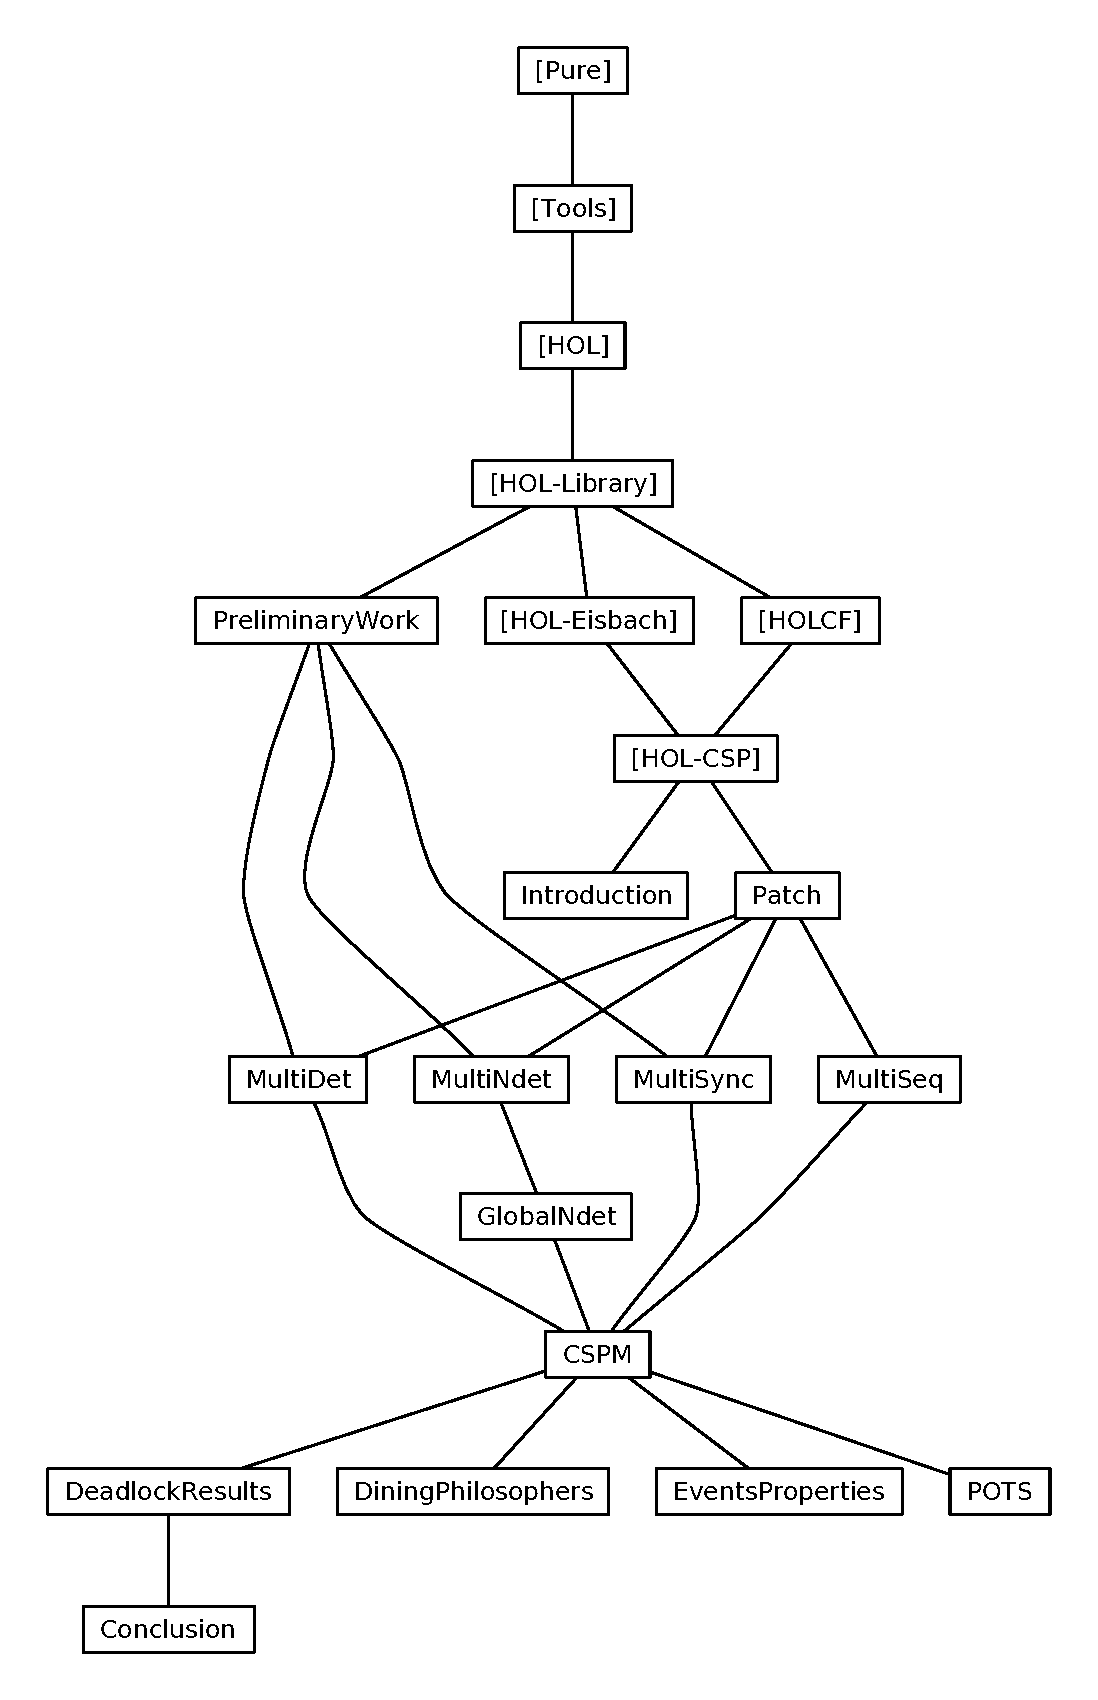
\includegraphics[width=0.2\textwidth,keepaspectratio]{session_graph}
\end{center}
\caption{Theory dependency graph}
\label{fig:thys}
\end{figure}

\newpage

% generated text of all theories
\input{session}

% optional bibliography
\bibliographystyle{alpha}
\bibliography{root}

\end{document}
